\section{Question 2}
\subsection{}
See code.

\subsection{}
For every call to device\_graph\_propagate we write one float and read 1 unsigned integer and 2 floats for every edge of the current node.

Therefore the total number of bytes read is
\begin{equation}
total\_bytes = node(f + edge(u+2f))NUM\_ITERATIONS
\end{equation}
where $f$ is the size of a float and $u$ is the size of an unsigned integer in bytes.


\subsection{}
\begin{figure}[!ht]
	\centering
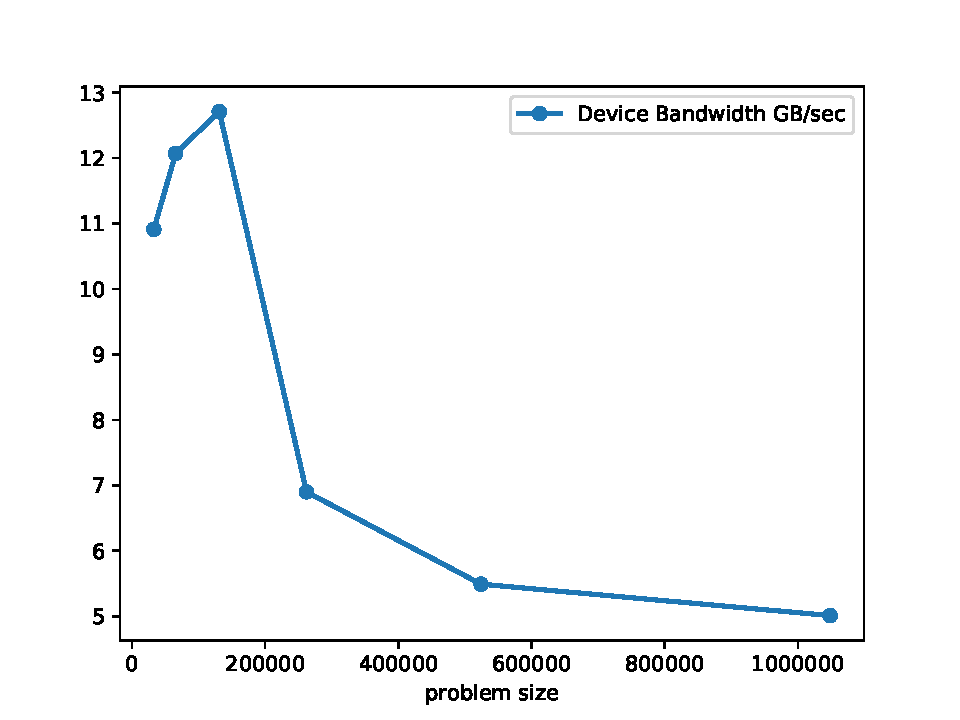
\includegraphics[scale=0.65]{graph.pdf}
\end{figure}

\subsection{}
For this problem, compared to problem 2, we are doing many more reads for each kernel call. The number of reads increases as the average edge size increases. This is reflected in the bandwidth measurements, where bandwidth decreases as average number of edges increases.

For example, with an average number of edges we are doing 31 reads and we get slightly more than 1/31 of the theoretical peak performance.

\tiny{\verbatiminput{../q2_results.txt}}
